\mysection{演習7}
\subsection{実行プログラム}
実行プログラムをソースコード\ref{s8}に示す。

\begin{lstlisting}[caption=演習7のプログラム,label=s8]
#include <stdio.h>
#include <dos.h>
#include "v25.h"
#include "ms.h"
  
int main()
{
  int s[3];
 
  pokeb(_V25BASE, _PMC0, 0x00); 
  pokeb(_V25BASE, _PM0, 0xff);  
 
  pokeb(_V25BASE, _PMC1, 0x20); 
      
  pokeb(_V25BASE, _PMC2, 0x00); 
  pokeb(_V25BASE, _PM2, 0xff); 
  
  printf("%c[2J", 0x1b); 
  while (1){
    ms_ifr(s); 
    printf("%c[01;01H", 0x1b); 
    printf("L:%d C:%d R:%d\n", s[0], s[1], s[2]); 
  }
  return 0;
}
\end{lstlisting}

\mysubsection{実行結果}
左右と真ん中に取り付けられた3つの近接センサの値(0か1)が出力される。

\mysection{演習8}
\subsection{実行プログラム}
実行プログラムは演習7と同様である。

\subsection{実行結果}
赤外線センサの2次元的な範囲を図\ref{niji}に示す。
扇型の外側が0の値を示す。(検知範囲外である。)
斜線部と白抜きを含めた扇型の内側の範囲がセンサの検知範囲であり、
白抜きが1の検知範囲、斜線部が0と1の間でばらつきがある範囲である。

\begin{figure}[H]
  \begin{center}
  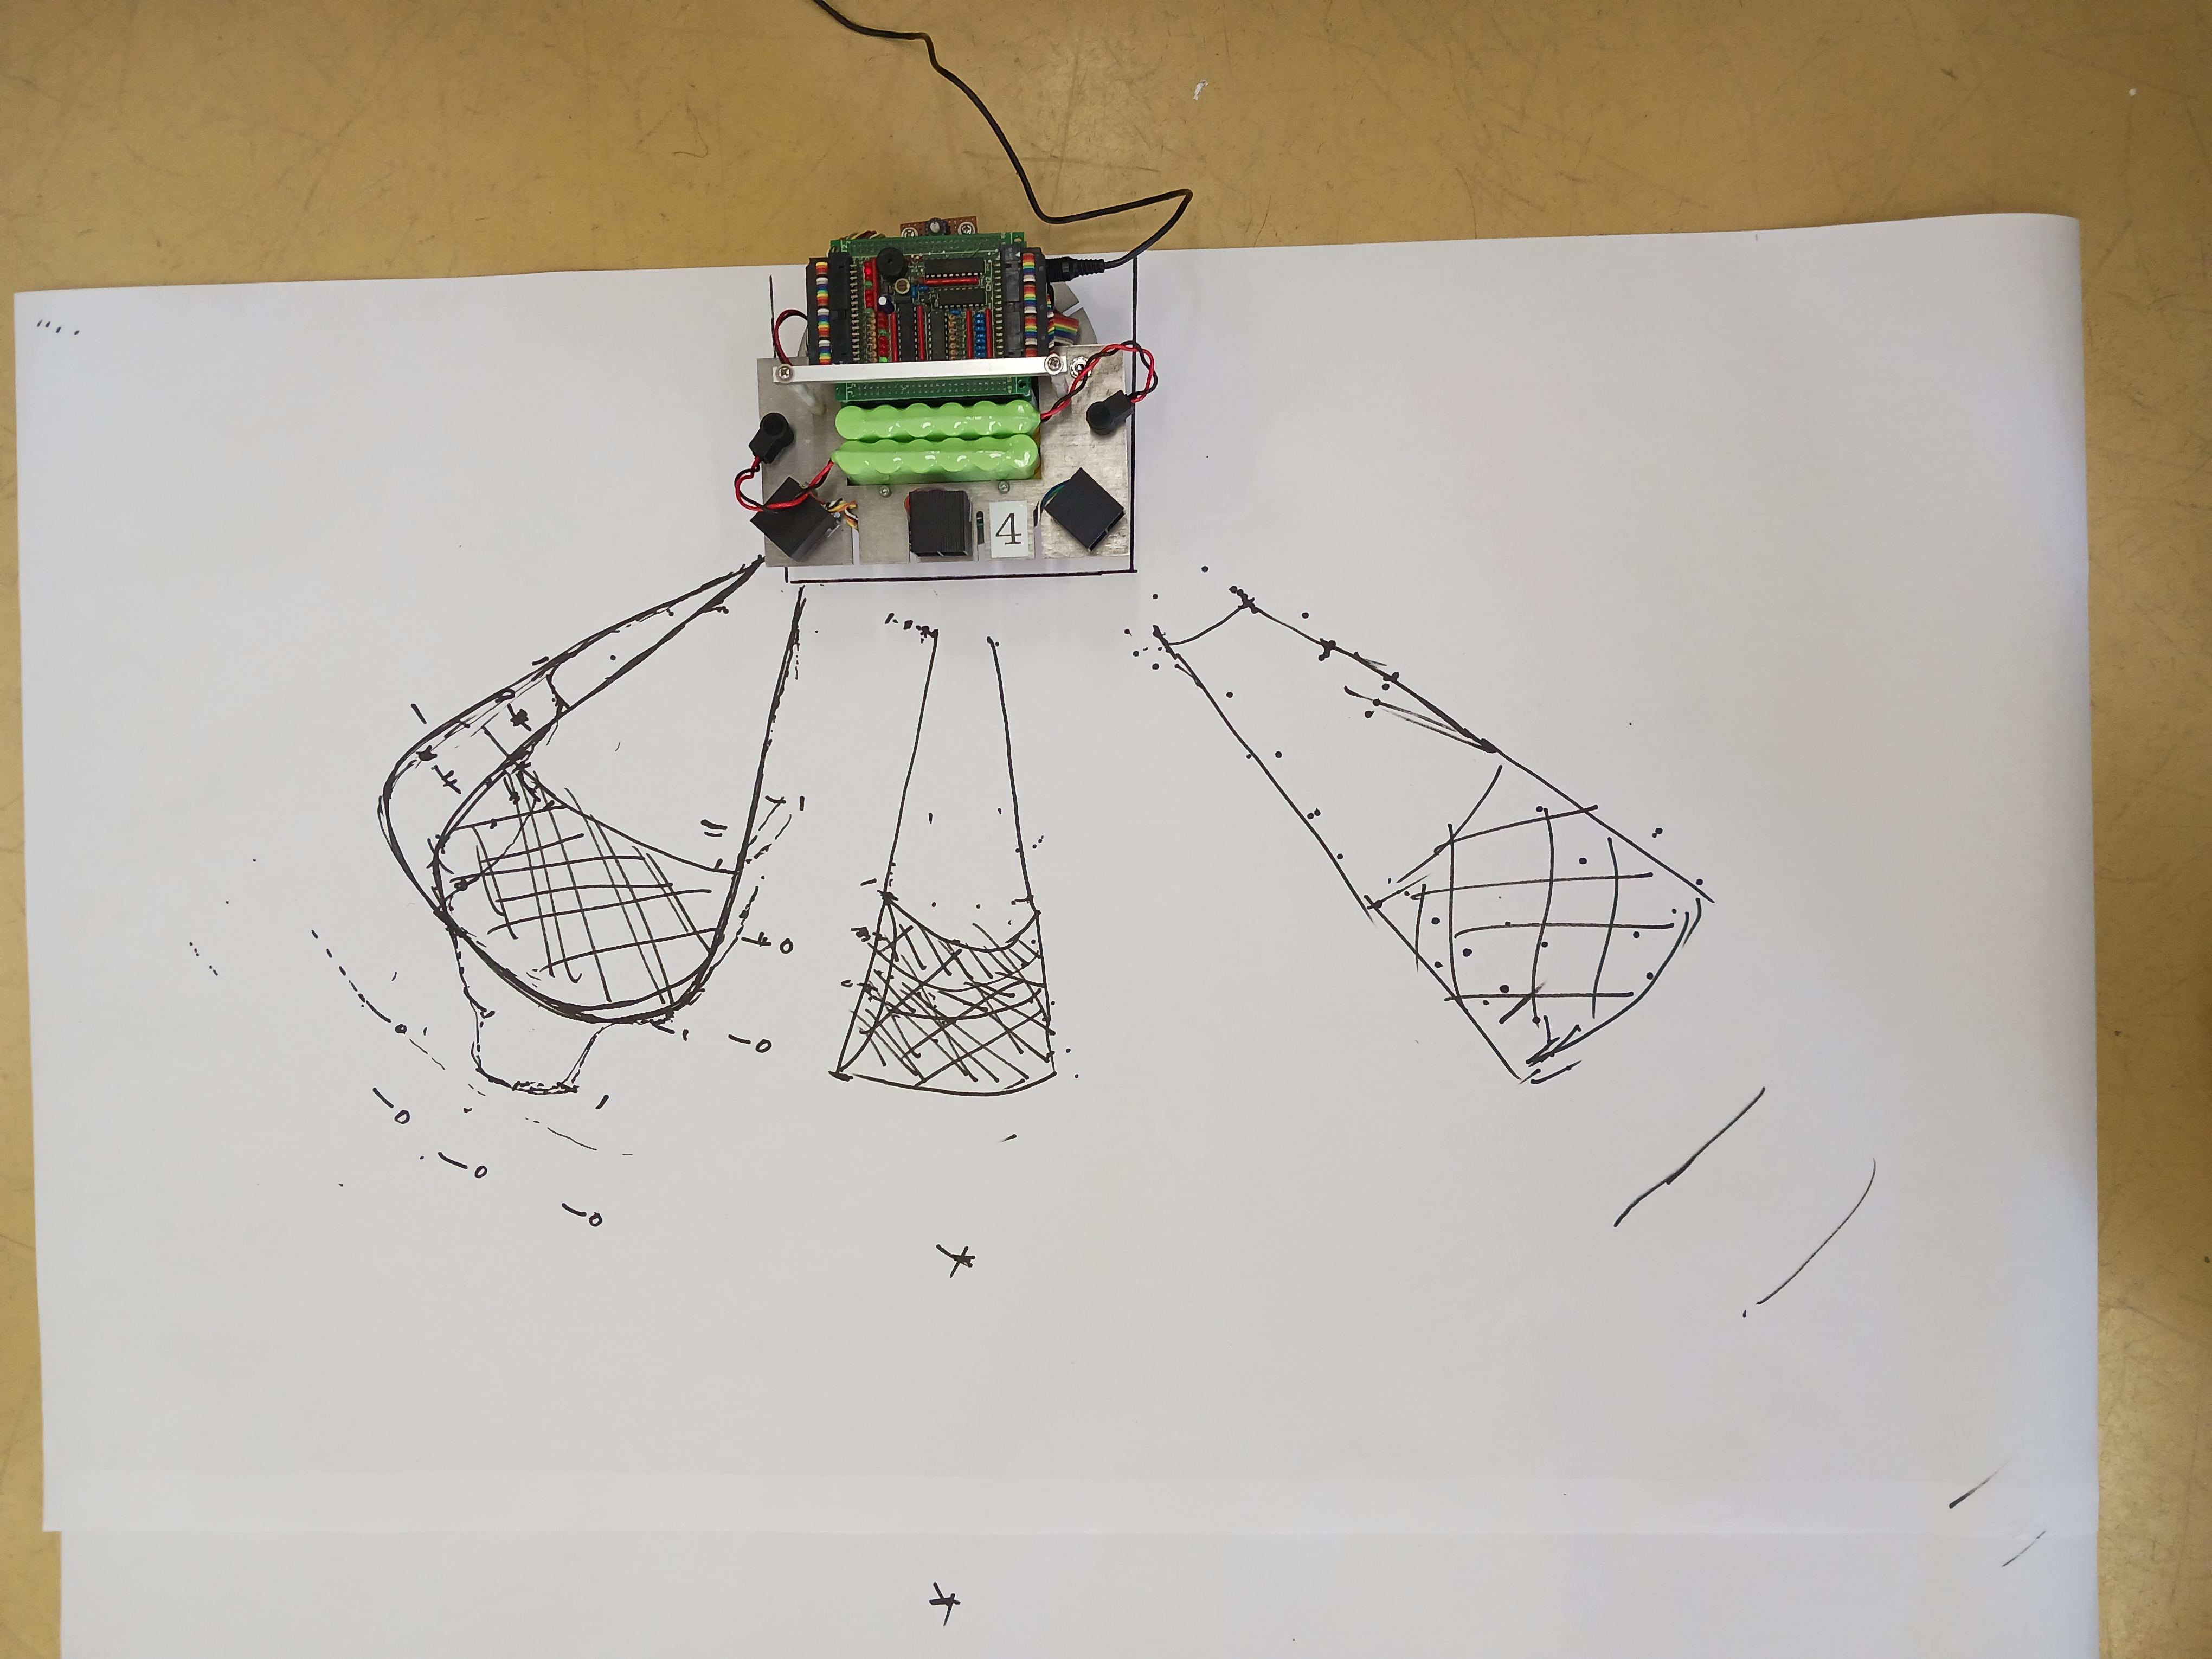
\includegraphics[width=.8\columnwidth]{img/8.jpg}
  \caption{赤外線センサの2次元的な範囲}
  \label{niji}
  \end{center}
\end{figure}

\section{演習9}
\subsection{実行プログラム}
実行プログラムをソースコード\ref{s9}に示す。
\begin{lstlisting}[caption=演習9のプログラム,label=s9]
#include <stdio.h>
#include <dos.h>
#include "v25.h"
#include "ms.h"
  
int main(){
  long cl, cr, ct;
  
  ms_enc_init();
  printf("%c[2J", 0x1b);
  while(1){
     ms_read_c(&cl, &cr, &ct);
  
    printf("%c[01;01H", 0x1b);
    printf("L:%10ld\n", cl);
    printf("R:%10ld\n", cr);
    printf("T:%10ld\n", ct);
  }
  return 0;
}
\end{lstlisting}

\subsection{実行結果}
タイヤを正回転させることで、
左右のモータのロータリーエンコーダの値が加算されて出力される。
タイヤを逆回転させると、減算されて出力される。

\section{演習10}
\subsection{実行プログラム}
実行プログラムをソースコード\ref{s10}に示す。
\begin{lstlisting}[caption=演習10のプログラム,label=s10]
#include <stdio.h>
#include <dos.h>
#include "v25.h"
#include "ms.h"
  
int main(){
  int i;
  long cl, cr, ct;
  long f[3] = {0, 0, 1};
  long f_old[3] = {0, 0, 0};
  float a_l, a_r, v_l, v_r;
  
  ms_enc_init();
  printf("%c[2J", 0x1b);
  while(1){
    ms_read_c(&cl, &cr, &ct);
  
    f[0] = cl;
    f[1] = cr;
    f[2] = ct*3/1000;
  
  
    a_l = (1000/3)*(f[0] - f_old[0])/(400*19.225);
    a_r = (1000/3)*(f[1] - f_old[1])/(400*19.225);
    v_l = (60*a_l);
    v_r = (60*a_r);
  
    printf("%c[01;01H", 0x1b);
    printf("a_l:%10lf\n", a_l);
    printf("a_r:%10lf\n", a_r);
    printf("v_l:%10lf\n", v_l);
    printf("v_r:%10lf\n", v_r);
          
    printf("T:%10ld\n", ct*3/1000);
  
    for (i = 0; i < 2; i++){
      f_old[i] = f[i];
    }
 
  }
  return 0;
}
\end{lstlisting}

\subsection{実行結果}
左右のロータリーエンコーダの値をモータの回転数に変換され、
モータの回転数の瞬時値が出力される。
